\documentclass[12pt]{article}
\usepackage[utf8]{inputenc}
\usepackage{amsmath,amssymb}
\usepackage{float}
\usepackage{graphicx}
\usepackage[a4paper, margin=2cm]{geometry}
\usepackage{enumerate}
\usepackage{xcolor}
\usepackage{caption}
% Definir un comando para el número de pregunta en azul
\newcommand{\question}[1]{\textcolor{blue}{\textbf{#1}}}
%\usepackage[spanish]{babel}
\begin{document}
\begin{titlepage}
        \begin{center}
            \LARGE \textbf{Taller No. 3\\Teoría Electromagnética}
            \vfill
            \large

            Karen Alejandra Freire Rosero\\
            Sonier Andrés Ortiz Castelblanco\\
            Sarah Isabel Tejada García\\
            Santiago Alejandro Pérez Ramos
            \vfill
            \textbf{Asignatura:} Teoría Electromagnética\\
            \textbf{Profesor:} Servio Tulio Pérez Merchancano, Ph.D\\
            \vfill
            Universidad del Cauca\\
            Facultad de Ciencias Naturales, Exactas y de la Educación\\
            Departamento de Física\\
            Popayán, Cauca\\
            2025
        \end{center}
\end{titlepage}
%----------------------------------------EJ_MDBL-----------------------------------------
\section*{\question{ Problema 1.11}} Encontrar los gradientes de las siguientes funciones:
\begin{enumerate}[(a)]
    
    \item \( f(x,y,z) = x^2 + y^3 + z^4 \)  
    \item \( f(x,y,z) = x^2 y^3 z^4 \) 
    \item \( f(x,y,z) = e^x \sin(y) \ln(z) \)

\end{enumerate}

Gradiente\\
\[
\fbox{ $\nabla f = \frac{\partial}{\partial x} \hat{i} + \frac{\partial}{\partial y} \hat{j} + \frac{\partial}{\partial z} \hat{k}$ }
\]

Desarrollando cada función\\

\textbf{(a)} \( \mathbf{f(x,y,z) = x^2 + y^3 + z^4} \)
\[
\nabla f(x,y,z) = \left( \frac{\partial}{\partial x} + \frac{\partial}{\partial y} + \frac{\partial}{\partial z} \right) (x^2 + y^3 + z^4)
\]

\begin{align*}
                &= \hat{i} \frac{\partial}{\partial x} (x^2 + y^3 + z^4) 
                 + \hat{j} \frac{\partial}{\partial y} (x^2 + y^3 + z^4) 
                 + \hat{k} \frac{\partial}{\partial z} (x^2 + y^3 + z^4) \\
                &=\boxed{ 2x \hat{i} + 3y^2 \hat{j} + 4z^3 \hat{k}}
\end{align*}

\textbf{(b) } \( \mathbf{f(x, y, z) = x^2y^3z^4} \)

\[
\nabla f(x,y,z) = \left( \frac{\partial}{\partial x} + \frac{\partial}{\partial y} + \frac{\partial}{\partial z} \right) (x^2 y^3 z^4)
\]

\begin{align*}
    =& \hat{i} \frac{\partial}{\partial x} (x^2 y^3 z^4) + \hat{j} \frac{\partial}{\partial y} (x^2 y^3 z^4) + \hat{k} \frac{\partial}{\partial z} (x^2 y^3 z^4) \\
    =&\boxed{ 2x y^3 z^4 \hat{i}  + 3x^2 y^2 z^4 \hat{j}  + 4x^2 y^3 z^3 \hat{k}} 
\end{align*}

\textbf{(c) } \( \mathbf{f(x,y,z) = e^x \sin(y) \ln(z)} \)

\[
\nabla f(x, y, z) = \left( \frac{\partial}{\partial x} \hat{x} + \frac{\partial}{\partial y} \hat{y} + \frac{\partial}{\partial z} \hat{z} \right) \left( e^x \sin(y) \ln(z) \right)
\]
\[
 = \fbox{$ e^x \sin(y) \ln(z) \hat{i} + e^x \cos(y) \ln(z) \hat{j} + e^x \sin(y) \left( \frac{1}{z} \right) \hat{k} $}
\]



\section*{\question{Problema 1.12}} La altura de una determinada colina (en pies) está dada por:
\[
h(x,y) = 10 \left( 2xy - 3x^2 - 4y^2 - 18x + 28y + 12 \right)
\]

donde \( y \) es la distancia (en millas) al norte y \( x \) la distancia al este de South Hadley.

\begin{enumerate}[(a)]
    \item ¿Dónde está ubicada la cima de la colina?
    \item ¿Qué altura tiene la colina?
    \item ¿Qué tan inclinada es la pendiente (en pies por milla) en el punto ubicado 7 millas al norte y 1 milla al este de South Hadley? ¿En qué dirección es más inclinada la pendiente en ese punto?
\end{enumerate}

Solución: 

\textbf{(a)}
La cima se encuentra donde el gradiente \( \nabla h \) es igual a cero:

\[\nabla h(x,y) = \left( \frac{\partial h}{\partial x}, \frac{\partial h}{\partial y} \right)\]

Calculamos las derivadas parciales:

\[\frac{\partial h}{\partial x} = 10 (2y - 6x - 18)\]

\[\frac{\partial h}{\partial y} = 10 (2x - 8y + 28)\]

Igualamos a cero:

\[2y - 6x - 18 = 0 \quad \Rightarrow \quad y - 3x = 9\]

\[2x - 8y + 28 = 0 \quad \Rightarrow \quad x - 4y = -14\]

Resolviendo el sistema:

\[x = 4(9 + 3x) - 14\]

\[x - 36 - 12x = -14\]

\[-17x = -14 + 36\]

\[x = \frac{22}{-11} = -2\]

Sustituyendo en la primera ecuación:

\[y = 9 + 3(-2)\]

\[y = 9 - 6 = 3\]

Por lo tanto, la cima está ubicada en:

\[\fbox{$ (x,y) = (-2,3) $ }\]

\textbf{(b)} Para hallar la altura de la colina evaluamos la función en \( h(-2,3) \):

\[h(-2,3) = 10 \left( -12 -12 + 36 + 36 + 84 + 12 \right)\]

\[= 10 (72) = 720\]

Por lo tanto, la altura de la colina es:\[ \fbox{$ \mathbf{720} \text{ pies.} $}\]

\section*{ \question{Problema 1.14}} Supongamos que \( f \) es una función de dos variables \( (y, z) \). Demuestra que el gradiente:  

\[
\nabla f = \left( \frac{\partial f}{\partial y} \right) \hat{y} + \left( \frac{\partial f}{\partial z} \right) \hat{z}
\]

se transforma como un vector bajo rotaciones:

\[
\frac{\partial f}{\partial \tilde{y}} = \left( \frac{\partial f}{\partial y} \right) \left( \frac{\partial y}{\partial \tilde{y}} \right) + \left( \frac{\partial f}{\partial z} \right) \left( \frac{\partial z}{\partial \tilde{y}} \right)
\]

y de forma análoga:

\[
\frac{\partial f}{\partial \tilde{z}}
\]

Sabemos que:

\[
\tilde{y} = y \cos \phi + z \sin \phi
\]

\[
\tilde{z} = -y \sin \phi + z \cos \phi
\]

Resolver estas ecuaciones para \( y \) y \( z \) en términos de \( \tilde{y} \) y \( \tilde{z} \), y calcular las derivadas necesarias:

\[
\frac{\partial y}{\partial \tilde{y}}, \quad \frac{\partial z}{\partial \tilde{y}}, \quad \text{etc.}
\]

Solución:

Dado que tenemos las ecuaciones \( \tilde{y} \) y \( \tilde{z} \) en términos de \( y, z \),  
obtenemos las ecuaciones para \( y, z \) usando la inversa:

\[
\begin{bmatrix}
y \\
z
\end{bmatrix}
=
\begin{bmatrix}
\cos\phi & -\sin\phi \\
\sin\phi & \cos\phi
\end{bmatrix}
\begin{bmatrix}
\tilde{y} \\
\tilde{z}
\end{bmatrix}
\]

La matriz de rotación es ortogonal, por lo que su inversa es su transpuesta:

\[
y = \tilde{y} \cos\phi - \tilde{z} \sin\phi
\]

\[
z = \tilde{y} \sin\phi + \tilde{z} \cos\phi
\]

Hallando las derivadas parciales

\[
\frac{\partial y}{\partial \tilde{y}} = \cos\phi, \quad \frac{\partial z}{\partial \tilde{y}} = \sin\phi
\]

\[
\frac{\partial y}{\partial \tilde{z}} = -\sin\phi, \quad \frac{\partial z}{\partial \tilde{z}} = \cos\phi
\]

Reemplazamos en la regla de la cadena

\[
\frac{\partial f}{\partial \tilde{y}} = \left( \frac{\partial f}{\partial y} \right) \cos\phi + \left( \frac{\partial f}{\partial z} \right) \sin\phi
\]

\[
\frac{\partial f}{\partial \tilde{z}} = \left( \frac{\partial f}{\partial y} \right) (-\sin\phi) + \left( \frac{\partial f}{\partial z} \right) \cos\phi
\]

Reescribiendo el gradiente

\[
\nabla f = \left( \frac{\partial f}{\partial \tilde{y}} \right) \hat{y} + \left( \frac{\partial f}{\partial \tilde{z}} \right) \hat{z}
\]

\[ 
\fbox{$\nabla f = \left(\frac{\partial f}{\partial y} \cos\phi + \frac{\partial f}{\partial z} \sin\phi \right) \hat{y} +
\left( -\frac{\partial f}{\partial y} \sin\phi + \frac{\partial f}{\partial z} \cos\phi \right) \hat{z}
$} \]\\


\section*{\question{Problema 1.16}} Dibuje la función vectorial \[
\mathbf{V} = \frac{\hat{r}}{r^2}
\]
y calcule su divergencia. Explique la respuesta.\\

Solución: \\
Esto representa un campo radial que apunta en la dirección de \( \hat{r} \) y cuya magnitud decrece con el cuadrado de la distancia. Descriendo un campo que se aleja del origen (si el signo es positivo) o converge hacia él (si el signo es negativo).

\begin{flushleft}
$\mathbf{V} \rightarrow$ campo radial \\  
$\hat{r} \rightarrow$ vector unitario \\  
$\mathbf{r} \rightarrow$ vector posición  
\end{flushleft}

Donde:

\[
r = \sqrt{x^2 + y^2 + z^2}, \quad r^2 = x^2 + y^2 + z^2
\]

\[
\hat{r} = \left( \frac{x}{r}, \frac{y}{r}, \frac{z}{r} \right)
\]
Reescribimos $\mathbf{V}$,  

\[
\mathbf{V} = \left( \frac{x}{r^3}, \frac{y}{r^3}, \frac{z}{r^3} \right)
\]
Calculando la divergencia, 
\[
\nabla \cdot \mathbf{V} = \frac{\partial}{\partial x} \left( \frac{x}{r^3} \right) + \frac{\partial}{\partial y} \left( \frac{y}{r^3} \right) + \frac{\partial}{\partial z} \left( \frac{z}{r^3} \right)
\]

Derivando usando la regla del cociente y sabiendo que:

\[
r^3 = (x^2 + y^2 + z^2)^{3/2}
\]

\[
\frac{\partial}{\partial x} \left( \frac{x}{r^3} \right) =
\frac{(1)r^3 - x \left( 3r^2 \frac{x}{r} \right)}{(r^3)^2}
\]

\[
\frac{\partial}{\partial x} \left( \frac{x}{r^3} \right) =
\frac{r^2 - 3x^2}{r^5}
\]

De igual forma para \( \frac{\partial}{\partial y} \left( \frac{y}{r^3} \right) \), \( \frac{\partial}{\partial z} \left( \frac{z}{r^3} \right) \):

\[
\frac{\partial}{\partial y} \left( \frac{y}{r^3} \right) =
\frac{r^2 - 3y^2}{r^5}
\]

\[
\frac{\partial}{\partial z} \left( \frac{z}{r^3} \right) =
\frac{r^2 - 3z^2}{r^5}
\]

Finalmente tenemos,  

\[
\nabla \cdot \mathbf{V} =
\frac{r^2 - 3x^2}{r^5} +
\frac{r^2 - 3y^2}{r^5} +
\frac{r^2 - 3z^2}{r^5}
\]

\[
= \frac{3r^2 - 3(x^2 + y^2 + z^2)}{r^5} =
\frac{3r^2 - 3r^2}{r^5} =
\frac{0}{r^5} = \fbox{$ 0$}
\]

La divergencia del campo es cero en todas partes excepto en el origen. Este origen actúa como fuente puntual del campo, descrita por la delta de Dirac.


\section*{ \question{Problema 1.18}}  Calcula el rotacional de las funciones vectoriales

\begin{align*}
\mathbf{V}_a &= x \hat{\mathbf{x}} + 3xz^2 \hat{\mathbf{y}} - 2xz \hat{\mathbf{z}} \\
\mathbf{V}_b &= xy \hat{\mathbf{x}} + 2yz \hat{\mathbf{y}} + 3zx \hat{\mathbf{z}} \\
\mathbf{V}_c &= y^2 \hat{\mathbf{x}} + (2xy + z) \hat{\mathbf{y}} + 2yz \hat{\mathbf{z}}
\end{align*}

Definición del rotacional
\[
\nabla \times \mathbf{V} =
\begin{vmatrix}
\hat{\mathbf{x}} & \hat{\mathbf{y}} & \hat{\mathbf{z}} \\
\frac{\partial}{\partial x} & \frac{\partial}{\partial y} & \frac{\partial}{\partial z} \\
V_x & V_y & V_z
\end{vmatrix}
\]

Cálculo del rotacional para $\mathbf{V}_a$
\[
\nabla \times \mathbf{V}_a =
\begin{vmatrix}
\hat{\mathbf{x}} & \hat{\mathbf{y}} & \hat{\mathbf{z}} \\
\frac{\partial}{\partial x} & \frac{\partial}{\partial y} & \frac{\partial}{\partial z} \\
x & 3xz^2 & -2xz
\end{vmatrix}
\]

\[
(\nabla \times \mathbf{V}_a)_x =
\frac{\partial (-2xz)}{\partial y} - \frac{\partial (3xz^2)}{\partial z} = 0 - 6xz = -6xz
\]

\[
(\nabla \times \mathbf{V}_a)_y =
\frac{\partial (x^2)}{\partial z} - \frac{\partial (-2xz)}{\partial x} = 0 + 2z = 2z
\]

\[
(\nabla \times \mathbf{V}_a)_z =
\frac{\partial (3xz^2)}{\partial x} - \frac{\partial (x^2)}{\partial y} = 3z^2 - 0 = 3z^2
\]

\[\fbox{$
\nabla \times \mathbf{V}_a = -6xz \hat{\mathbf{x}} + 2z \hat{\mathbf{y}} + 3z^2 \hat{\mathbf{z}}$}
\]

Cálculo del rotacional para $\mathbf{V}_b$
\[
\nabla \times \mathbf{V}_b =
\begin{vmatrix}
\hat{\mathbf{x}} & \hat{\mathbf{y}} & \hat{\mathbf{z}} \\
\frac{\partial}{\partial x} & \frac{\partial}{\partial y} & \frac{\partial}{\partial z} \\
xy & 2yz & 3zx
\end{vmatrix}
\]

\[
\nabla \times \mathbf{V}_b =
\hat{\mathbf{x}} (0 - 2y) +
\hat{\mathbf{y}} (0 - 3z) +
\hat{\mathbf{z}} (0 - x)
\]

\[\fbox{$
\nabla \times \mathbf{V}_b = -2y \hat{\mathbf{x}} - 3z \hat{\mathbf{y}} - x \hat{\mathbf{z}}$}
\]

Cálculo del rotacional para $\mathbf{V}_c$
\[
\nabla \times \mathbf{V}_c =
\begin{vmatrix}
\hat{\mathbf{x}} & \hat{\mathbf{y}} & \hat{\mathbf{z}} \\
\frac{\partial}{\partial x} & \frac{\partial}{\partial y} & \frac{\partial}{\partial z} \\
y^2 & (2xy+z^2) & 2yz
\end{vmatrix}
\]

\[
= \hat{\mathbf{x}} (2z - 2z) + \hat{\mathbf{y}} (0 - 0) + \hat{\mathbf{z}} (2y - 2y) \]

\[\fbox{$
\nabla \times \mathbf{V}_c=0$}
\]

\section*{ \question{Problema 1.20}}  Construir una función vectorial que tenga cero divergencia y cero rotacional.

\[
\mathbf{V}_a = y \hat{\mathbf{x}} + x \hat{\mathbf{y}}
\]

\[
\mathbf{V}_b = yz \hat{\mathbf{x}} + xz \hat{\mathbf{y}} + xy \hat{\mathbf{z}}
\]

\[
\mathbf{V}_c = (3x^2z - z^3) \hat{\mathbf{x}} + 3y \hat{\mathbf{y}} + (x^3 - 3xz^2) \hat{\mathbf{z}}
\]

Cálculo de la divergencia,\\

Para $\mathbf{V}_a$:
\[
\nabla \cdot \mathbf{V}_a = \frac{\partial y}{\partial x} + \frac{\partial x}{\partial y}  = 0
\]

Para $\mathbf{V}_b$:
\[
\nabla \cdot \mathbf{V}_b = \frac{\partial yz}{\partial x} + \frac{\partial xz}{\partial y} + \frac{\partial xy}{\partial z} = 0
\]

Para $\mathbf{V}_c$:
\[
\nabla \cdot \mathbf{V}_c = \frac{\partial (3x^2z - z^3)}{\partial x} + \frac{\partial 3y}{\partial y} + \frac{\partial (x^3 - 3xz^2)}{\partial z}
\]

\[= 6xz + 0 - 6xz = 0\]

Cálculo del rotacional,\\

\[
\nabla \times \mathbf{V}_a = \left( \frac{\partial 0}{\partial y} - \frac{\partial x}{\partial z} \right) - \left( \frac{\partial y}{\partial z} - \frac{\partial 0}{\partial x} \right) - \left( \frac{\partial x}{\partial x} - \frac{\partial y}{\partial y} \right)
\]

\[= 0 - 0 - (1 - 1) = 0\]

\[
\nabla \times \mathbf{V}_b = \left( \frac{\partial xy}{\partial y} - \frac{\partial xz}{\partial z} \right) - \left( \frac{\partial xy}{\partial x} - \frac{\partial yz}{\partial z} \right) + \left( \frac{\partial xz}{\partial x} - \frac{\partial yz}{\partial y} \right)
\]

\[= (x - x) - (y - y) + (z - z) = 0\]

\[
\nabla \times \mathbf{V}_c = \left( \frac{\partial}{\partial y} (x^3 - 3x z^2)  - \frac{\partial 3}{\partial z}\right) - \left( \frac{\partial}{\partial x} (x^3 - 3x z^2) - \frac{\partial}{\partial z} (3x^2 z - z^3) \right) + \left( \frac{\partial 3}{\partial x} - \frac{\partial}{\partial y} (3x^2 z - z^3) \right)
\]

\[= (0 - 0) - \left[ (3x^2 - 3z^2) - (3x^2 - 3z^2) \right] + (0 - 0) = 0\]\\

\section*{ \question{Problema 1.22}} Si \(\mathbf{A}\) y \(\mathbf{B}\) son dos funciones vectoriales, ¿qué significa la expresión \((\mathbf{A} \cdot \nabla) \mathbf{B}\)?

Es decir, ¿cuáles son sus componentes \(x\), \(y\) y \(z\) en términos de las componentes cartesianas de \(\mathbf{A}\), \(\mathbf{B}\) y \(\nabla\)?

\[
\mathbf{A} = (A_x, A_y, A_z)
\]

\[
\mathbf{B} = (B_x, B_y, B_z)
\]

\[
\nabla = \left( \frac{\partial}{\partial x}, \frac{\partial}{\partial y}, \frac{\partial}{\partial z} \right)
\]

\[
(\mathbf{A} \cdot \nabla) \mathbf{B} = \left[ A_x \frac{\partial}{\partial x} + A_y \frac{\partial}{\partial y} + A_z \frac{\partial}{\partial z} \right] 
\begin{bmatrix} B_x \\ B_y \\ B_z \end{bmatrix}
\]

\[
= 
\begin{bmatrix}
A_x \frac{\partial B_x}{\partial x} + A_y \frac{\partial B_x}{\partial y} + A_z \frac{\partial B_x}{\partial z} \\
A_x \frac{\partial B_y}{\partial x} + A_y \frac{\partial B_y}{\partial y} + A_z \frac{\partial B_y}{\partial z} \\
A_x \frac{\partial B_z}{\partial x} + A_y \frac{\partial B_z}{\partial y} + A_z \frac{\partial B_z}{\partial z}
\end{bmatrix}
\]

\[(\mathbf{A} \cdot \nabla) \mathbf{B} = \left( A_x \frac{\partial B_x}{\partial x} + A_y \frac{\partial B_x}{\partial y} + A_z \frac{\partial B_x}{\partial z} \right) \hat{x} +
\]

\[
\left( A_x \frac{\partial B_y}{\partial x} + A_y \frac{\partial B_y}{\partial y} + A_z \frac{\partial B_y}{\partial z} \right) \hat{y} +
\]

\[
\left( A_x \frac{\partial B_z}{\partial x} + A_y \frac{\partial B_z}{\partial y} + A_z \frac{\partial B_z}{\partial z} \right) \hat{z}
\]

\textbf{(b)} Calcula\quad \( (\mathbf{r} \cdot \nabla) \hat{r} \), donde \(\hat{\mathbf{r}}\) es el vector unitario definido en la Ec. 1.21.\\

Sabemos que:
\[
\hat{r} = \frac{\mathbf{r}}{r} = \frac{x}{r} \hat{i} + \frac{y}{r} \hat{j} + \frac{z}{r} \hat{k}
\]

\[
( \hat{\mathbf{r}} \cdot \nabla) \hat{r} = \left( \frac{x}{r} \frac{\partial}{\partial x} + \frac{y}{r} \frac{\partial}{\partial y} + \frac{z}{r} \frac{\partial}{\partial z} \right) 
\begin{bmatrix} \frac{x}{r} \\ \frac{y}{r} \\ \frac{z}{r} \end{bmatrix}
\]

\[
[(\hat{\mathbf{r}} \cdot \nabla) \hat{r}]_x = \frac{x}{r} \frac{\partial}{\partial x} \left( \frac{x}{r} \right) + \frac{y}{r} \frac{\partial}{\partial y} \left( \frac{x}{r} \right) + \frac{z}{r} \frac{\partial}{\partial z} \left( \frac{x}{r} \right)
\]

\[
= \frac{1}{r}\left( x \frac{\partial }{\partial x} + y \frac{\partial}{\partial y} \left( \frac{x}{r} \right) + z \frac{\partial}{\partial z} \left( \frac{x}{r} \right)\right)
\]

Resolviendo cada derivada parcial:

\[
\frac{\partial}{\partial x} \left( \frac{x}{\sqrt{x^2 + y^2 + z^2}} \right) = \frac{r - x \cdot \left( \frac{x}{r} \right)}{r^2} = \frac{r - \frac{x^2}{r}}{r^2} = \frac{r^2 -x^2}{r^3}
\]

\[
\frac{\partial}{\partial y} \left( \frac{x}{r} \right) =\frac{ 0 - x \cdot \left( \frac{y}{r} \right)}{r^2} = -\frac{xy}{r^3}
\]

\[
\frac{\partial}{\partial z} \left( \frac{x}{r} \right) =\frac{ 0 - x \cdot \left( \frac{z}{r} \right)}{r^2} = -\frac{xz}{r^3}
\]
Resolviendo para la componente en x,
\[
[(\hat{\mathbf{r}} \cdot \nabla) \hat{r}]_x = \frac{1}{r} \left[ x \left( \frac{r^2 -x^2}{r^3} \right) + y \left( -\frac{xy}{r^3} \right) + z \left( -\frac{xz}{r^3} \right) \right]
\]


\[
= \frac{1}{r} \left[ \frac{x}{r} -  \frac{x}{r^3} (x^2 + y^2 + z^2) \right] = \frac{x}{r^2} - \frac{x \cdot r^2}{r^4} 
\]

\[
= \frac{x}{r^2} - \frac{x}{r^2} = 0 \quad 
\]

De igual forma para las demás componentes.  
De ahí que:

\[ \fbox{$
(\mathbf{r} \cdot \nabla) \hat{r} = 0 $} 
\]

\textbf{(c)} Para las funciones del Problema 1.15, evalúe \( (\mathbf{V}_a \cdot \nabla) \mathbf{V}_b \).
\[
\mathbf{V}_a = x^2 \hat{\mathbf{x}} + 3xz^2 \hat{\mathbf{y}} - 2xz \hat{\mathbf{z}}
\]

\[
\mathbf{V}_b = xy \hat{\mathbf{x}} + 2yz \hat{\mathbf{y}} + 3xz \hat{\mathbf{z}}
\]

\[
(\mathbf{V}_a \cdot \nabla) \mathbf{V}_b =
\begin{bmatrix}
x^2 \frac{\partial}{\partial x} & 3x z^2 \frac{\partial}{\partial y} & -2xz \frac{\partial}{\partial z}
\end{bmatrix}
\begin{bmatrix}
xy \\ 2yz \\ 3xz
\end{bmatrix}
\]

\[
= \left( x^2 \frac{\partial}{\partial x} (xy \hat{\mathbf{x}} + 2yz \hat{\mathbf{y}} + 3zx \hat{\mathbf{z}} ) + 3xz^2 \frac{\partial}{\partial y} (xy \hat{\mathbf{x}} + 2yz \hat{\mathbf{y}}+ 3xz \hat{\mathbf{z}})- 2xz \frac{\partial}{\partial z} (xy \hat{\mathbf{x}}+ 2yz \hat{\mathbf{y}} + 3xz \hat{\mathbf{z}})\right) 
\]

\[
= x^2 \left( y \hat{\mathbf{x}}+ 0\hat{\mathbf{y}} + 3z\hat{\mathbf{z}} \right)  + 3xz^2 \left( x\hat{\mathbf{x}} + 2z\hat{\mathbf{y}} + 0\hat{\mathbf{z}} \right)- 2xz \left( 0\hat{\mathbf{x}} + 2y \hat{\mathbf{y}}+ 3x \hat{\mathbf{x}}\right)
\]

\[
= \left( x^2 y + 3x^2 z^2 \right) \hat{\mathbf{x}} + \left( 6xz^3 - 4xyz \right) \hat{\mathbf{y}} + \left( 3x^2 z - 6x^2 z \right) \hat{\mathbf{z}}
\]

\[\fbox{$
(\mathbf{V}_a \cdot \nabla) \mathbf{V}_b = x^2 (y + 3z^2) \hat{\mathbf{x}} + 2xz (3z^2 - 2y) \hat{\mathbf{y}} - 3x^2 z \hat{\mathbf{z}}
$}\]\\

\section*{\question{Problema 1.24}} Deriva las tres reglas del cociente

\[
\nabla \left( \frac{f}{g} \right) = \frac{\partial}{\partial x} \left( \frac{f}{g} \right) \hat{\mathbf{x}} + \frac{\partial}{\partial y} \left( \frac{f}{g} \right) \hat{\mathbf{y}} + \frac{\partial}{\partial z} \left( \frac{f}{g} \right) \hat{\mathbf{z}}
\]

\[
= \frac{g \frac{\partial f}{\partial x} - f \frac{\partial g}{\partial x}}{g^2} \hat{\mathbf{x}} + \frac{g \frac{\partial f}{\partial y} - f \frac{\partial g}{\partial y}}{g^2} \hat{\mathbf{y}} + \frac{g \frac{\partial f}{\partial z} - f \frac{\partial g}{\partial z}}{g^2} \hat{\mathbf{z}}
\]

\[
= \frac{1}{g^2} \left[ g \left( \frac{\partial f}{\partial x} \hat{x} + \frac{\partial f}{\partial y} \hat{y} + \frac{\partial f}{\partial z} \hat{z} \right) - f \left( \frac{\partial g}{\partial x} \hat{x} + \frac{\partial g}{\partial y} \hat{y} + \frac{\partial g}{\partial z} \hat{z} \right) \right]
\]

\[\fbox{$
= \frac{1}{g^2} \left[ g \nabla f - f \nabla g \right]$}
\]
Divergencia de un cociente,
\[
\nabla \cdot \left( \frac{\mathbf{A}}{g} \right) = \frac{\partial}{\partial x} \left( \frac{A_x}{g} \right) + \frac{\partial}{\partial y} \left( \frac{A_y}{g} \right) + \frac{\partial}{\partial z} \left( \frac{A_z}{g} \right)
\]

\[
= \frac{g \frac{\partial A_x}{\partial x} - A_x \frac{\partial g}{\partial x}}{g^2} + \frac{g \frac{\partial A_y}{\partial y} - A_y \frac{\partial g}{\partial y}}{g^2} + \frac{g \frac{\partial A_z}{\partial z} - A_z \frac{\partial g}{\partial z}}{g^2}
\]

\[
= \frac{1}{g^2} \left[ g \left( \frac{\partial Ax}{\partial x}  + \frac{\partial Ay}{\partial y}  + \frac{\partial Az}{\partial z}  \right) -  \left( Ax\frac{\partial g}{\partial x} + Ay\frac{\partial g}{\partial y}  + Az\frac{\partial g}{\partial z}  \right) \right]
\]

\[\fbox{$
= \frac{1}{g^2} \left[ g (\nabla \cdot \mathbf{A}) - \mathbf{A} \cdot \nabla g \right]$}
\]

Rotacional de un cociente,
\[
\left[ \nabla \times \left( \frac{\mathbf{A}}{g} \right) \right]_x = \left( \frac{\partial}{\partial y} \left( \frac{A_z}{g} \right) - \frac{\partial}{\partial z} \left( \frac{A_y}{g} \right) \right)
\]

\[
= \frac{g \frac{\partial A_z}{\partial y} - A_z \frac{\partial g}{\partial y}}{g^2} - \frac{g \frac{\partial A_y}{\partial z} - A_y \frac{\partial g}{\partial z}}{g^2}
\]

\[
= \frac{1}{g^2} \left[ g \left( \frac{\partial A_z}{\partial y} - \frac{\partial A_y}{\partial z} \right) - \left( A_z \frac{\partial g}{\partial y} - A_y \frac{\partial g}{\partial z} \right) \right]
\]

\[\fbox{$
= \frac{1}{g^2} \left[ g (\nabla \times \mathbf{A})_x - (\mathbf{A} \times \nabla g)_x \right] $}
\]

Del mismo modo para las componentes en \( y \) \textit{y} \( z \).


%----------------------------------------Fn_MDBL-----------------------------------------

%----------------------------------------EJ_ACCH--------------------------------
\section*{\question{Problema 1.26.}} Calcula el laplaciano de las siguientes funciones

\subsection*{(a) \( T_a = x^2 + 2xy + 3z + 4 \)}

Se tiene:
\[
\nabla^2 T_a = \left( \frac{\partial^2}{\partial x^2}\ + \frac{\partial^2}{\partial y^2}\ + \frac{\partial^2}{\partial z^2}  \right) (x^2 + 2xy + 3z + 4)
\]

Se determinan las primeras derivadas:

\[
\frac{\partial T_a}{\partial x} = 2x + 2y
\]

\[
\frac{\partial T_a}{\partial y} = 2x
\]

\[
\frac{\partial T_a}{\partial z} = 3
\]

Ahora:

\[
\frac{\partial^2 T_a}{\partial x^2} = 2
\]

\[
\frac{\partial^2 T_a}{\partial y^2} = 0
\]

\[
\frac{\partial^2 T_a}{\partial z^2} = 0
\]

Por lo tanto:

\[
\boxed{\nabla^2 T_a = 2 + 0 + 0 = 2}
\]

\subsection*{(b) \( T_b = \sin x \sin y \sin z \)}

\[
\nabla^2 T_b = \left( \frac{\partial^2}{\partial x^2}\ + \frac{\partial^2}{\partial y^2}+ \frac{\partial^2}{\partial z^2}  \right) ( \sin x \sin y \sin z )
\]

Se calculan las derivadas de primer orden:

\[
\frac{\partial T_b}{\partial x} = \cos x \sin y \sin z
\]

\[
\frac{\partial T_b}{\partial y} = \sin x \cos y \sin z
\]

\[
\frac{\partial T_b}{\partial z} = \sin x \sin y \cos z
\]

Ahora:

\[
\frac{\partial^2 T_b}{\partial x^2} = -\sin x \sin y \sin z
\]

\[
\frac{\partial^2 T_b}{\partial y^2} = -\sin x \sin y \sin z
\]

\[
\frac{\partial^2 T_b}{\partial z^2} = -\sin x \sin y \sin z
\]

Finalmente:

\[
\nabla^2 T_b = -\sin x \sin y \sin z - \sin x \sin y \sin z - \sin x \sin y \sin z
\]

\[
\boxed{\nabla^2 T_b = -3 \sin x \sin y \sin z}
\]

\subsection*{(c) \( T_c = e^{-5x} \sin 4y \cos 3z \)}

El laplaciano:

\[
 \left( \frac{\partial^2}{\partial x^2}\  + \frac{\partial^2}{\partial y^2}+ \frac{\partial^2}{\partial z^2} \right) \left( e^{-5x} \sin 4y \cos 3z \right)
\]
Primeras derivadas parciales:

\[
\frac{\partial T_c}{\partial x} = -5e^{-5x} \sin 4y \cos 3z
\]
\[
\frac{\partial T_c}{\partial y} = e^{-5x} \cos 4y \cos 3z \cdot 4
\]
\[
\frac{\partial T_c}{\partial z} = -e^{-5x} \sin 4y \sin 3z \cdot 3
\]
Segundas derivadas:
\[
\frac{\partial^2 T_c}{\partial x^2} = 25e^{-5x} \sin 4y \cos 3z
\]

\[
\frac{\partial^2 T_c}{\partial y^2} = -16e^{-5x} \sin 4y \cos 3z
\]


\[
\frac{\partial^2 T_c}{\partial z^2} = -9e^{-5x} \sin 4y \cos 3z
\]
Por tanto:
\[
\nabla^2 T_c = 25e^{-5x} \sin 4y \cos 3z - 16e^{-5x} \sin 4y \cos 3z - 9e^{-5x} \sin 4y \cos 3z
\]

\[
\boxed{\nabla^2 T_c = 0}
\]

\subsection*{(d) \( V = x^2 \hat{x} + 3x z^2 \hat{y} + 2xz \hat{z} \)}

El laplaciano para cada componente:

\[
\nabla^2 V = \left( \nabla^2 V_x \right) \hat{x} + \left( \nabla^2 V_y \right) \hat{y} + \left( \nabla^2 V_z \right) \hat{z}
\]


\[
\frac{\partial V_x}{\partial x} = 2x \hat{x}
\] \[
\frac{\partial^2 V_x}{\partial x^2} = 2
\]


\[
\frac{\partial V_y}{\partial y} = 0
\]

\[
\frac{\partial^2 V_y}{\partial y^2} = 0
\]

\[
\frac{\partial V_z}{\partial z} = 6xz\hat{y} - 2x\hat{z}
\]

\[
\frac{\partial^2 V_z}{\partial z^2} = 6x \hat{y}
\]

Por lo tanto, el laplaciano de \( V \) es:

\[
\boxed{\nabla^2 V = 2 \hat{x} + 6x \hat{y}}
\]

\section*{\question{Problema 1.28} }Demuestre que el rotacional de un gradiente siempre es cero. Compruébelo para la función (b) del 9.11.

\[
F(x,y,z) = x^2 y^3 z^4
\]

El rotacional de un gradiente es:

\[
\nabla \times (\nabla f) = 0
\]

Se calcula el gradiente de \( f \):

\[
\nabla f = \left( \frac{\partial}{\partial x} \hat{x} + \frac{\partial}{\partial y} \hat{y} + \frac{\partial}{\partial z} \hat{z} \right) (x^2 y^3 z^4)
\]

\[
\nabla f = 2x y^3 z^4 \hat{x} + 3x^2 y^2 z^4 \hat{y} + 4x^2 y^3 z^3 \hat{z}
\]

El rotacional:

\[
\nabla \times (\nabla f) =
\begin{vmatrix}
\hat{x} & \hat{y} & \hat{z} \\
\frac{\partial}{\partial x} & \frac{\partial}{\partial y} & \frac{\partial}{\partial z} \\
2x y^3 z^4 & 3x^2 y^2 z^4 & 4x^2 y^3 z^3
\end{vmatrix}
\]

Entonces:

\[
\nabla \times (\nabla f) = (12x y^2 z^3 - 12x y^2 z^3) \hat{x} - (8x y^3 z^3 - 8x y^3 z^3) \hat{y} + (6x y^ 2 z^4 - 6x y^2 z^4) \hat{z} 
\]

\[
\boxed{\nabla \times (\nabla f) = 0}
\]

\section*{\question{Problema  1.30}} Calcule la integral de superficie de la función en el Ej. 1.7 sobre la parte superior de la caja. ¿Depende la integral de superficie solo de la línea de frontera para esta función? ¿Cuál es el flujo total sobre la superficie cerrada de la caja incluyendo la parte inferior?

Función:

\[
V = 2x z \hat{x} + (x+2) \hat{y} + 4(z^2 - 3) \hat{z}
\]

Tenemos: \( z=0 \)

\[
da = -dxdy \hat{z}
\]

\[
V \cdot da = -y (z^3 -3) dxdy
\]

Como \( z=0 \):

\[
V \cdot da = -y(0-3)dxdy
\]

\[
V \cdot da = 3y dxdy
\]
Por lo que:
\[
\iint V \cdot da = \int_0^2 \int_0^2 3y dxdy
\]
Entonces:
\[
= \int_0^2 dx \int_0^2 3y dy
\]

\[
= \int_0^2 dx 3  \frac{y^2}{2}\Big|_0^2
\]

\[
= \int_0^2 dx 6
\]

\[
= 6 \int_0^2 dx = 6 x \Big|_0^2
\]

\[
\boxed{= 12}
\]
La integral de superficie no depende únicamente de la línea límite ya que En el ejemplo 1.7 se obtuvo 20 para la misma línea límite (el cuadrado en el plano xy).
 El flujo total sería: \[
    20 + 12 = \boxed{32}   \]

 \section*{\question{Problema  1.32}} Verificar el teorema fundamental para gradientes usando 

\[
T = x^2 + 4xy + 2y z^3
\]

los puntos \( a = (0,0,0) \) y \( b = (1,1,1) \) y las tres rutas de la figura 1.28.

\begin{enumerate}
    \item \( (0,0,0) \to (1,0,0) \to (1,1,0) \to (1,1,1) \)
    \item \( (0,0,0) \to (0,0,1) \to (0,1,1) \to (1,1,1) \)
    \item La trayectoria parabólica \( z = x^2 \), \( y = x \)
\end{enumerate}

\begin{figure}[h] 
    \centering
    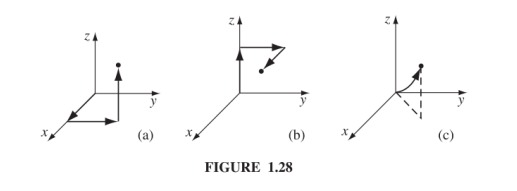
\includegraphics[width=0.7\textwidth]{imagenes/punto_28.jpg} 
    \label{fig:mi_figura}
\end{figure}


\textbf{Teorema Fundamental:}

\[
\int_a^b \nabla T \cdot d\mathbf{l} = T(b) - T(a)
\]

Se tiene:

\[
T(b) = 7
\]

\[
T(a) = 0 \quad \Rightarrow \quad T(0,0,0) = 0
\]

\[
\boxed{T(b) - T(a) = 7}
\]

Se calcula el gradiente de \( T \):

\[
\nabla T = \left( \frac{\partial}{\partial x} \hat{x} + \frac{\partial}{\partial y} \hat{y} + \frac{\partial}{\partial z} \hat{z} \right) (x^2 + 4xy + 2y z^3)
\]

\[
\nabla T = (2x + 4y) \hat{x} + (4x + 2z^3) \hat{y} + (6y z^2) \hat{z}
\]

Por otro lado:

\[
d\mathbf{l} = dx \hat{x} + dy \hat{y} + dz \hat{z}
\]
\[
\nabla T \cdot d\mathbf{l} = (2x + 4y)dx + (4x + 2z^3)dy + (6y z^2)dz
\]

\subsection*{Para la Primera Ruta (a):}

\textbf{En 1°:} \( x: 0 \to 1 \)

\[
y = 0, \quad z = 0
\]

\[
dy = 0, \quad dz = 0
\]

\[
\int \nabla T \cdot d\mathbf{l} = \int_0^1 2x \, dx = 2 \int_0^1 x \, dx
\]

\[
= 2 \left[ \frac{x^2}{2} \right]_0^1
\]

\[
= 2 \left( \frac{1}{2} \right) = 1
\]

\textbf{En 2°:} \( y: 0 \to 1 \)

\[
x = 1, \quad z = 0
\]

\[
dx = 0, \quad dy = 1
\]

\[
\int \nabla T \cdot d\mathbf{l} = \int_0^1 4 dy = 4 \int_0^1 dy
\]

\[
= 4 \left[ y \right]_0^1 = 4
\]

\textbf{En 3°:} \( z: 0 \to 1 \)

\[
y = 1, \quad x = 1
\]

\[
dx = 0, \quad dy = 0
\]

\[
\int \nabla T \cdot d\mathbf{l} = \int_0^1 6z^2 dz = 6 \int_0^1 z^2 dz
\]

\[
= 6 \left[ \frac{z^3}{3} \right]_0^1 = 6 \times \frac{1}{3} = 2
\]

\[
\int_a^b \nabla T \cdot d\mathbf{l} = 1 + 4 + 2 = \boxed{7}
\]


\subsection*{Para la Segunda Ruta (b):}

\textbf{En 1°:} \( z: 0 \to 1 \)

\[
y = 0, \quad x = 0
\]

\[
dx = 0, \quad dy = 0
\]

\[
\int \nabla T \cdot d\mathbf{l} = 0
\]

\textbf{En 2°:} \( y: 0 \to 1 \)

\[
x = 0, \quad z = 1
\]

\[
dx = 0, \quad dz = 0
\]

\[
\int \nabla T \cdot d\mathbf{l} = \int_0^1 2 \, dy = 2 \int_0^1 dy = 2
\]

\textbf{En 3°:} \( x: 0 \to 1 \)

\[
y = 1, \quad z = 1
\]

\[
dy = 0, \quad dz = 0
\]

\[
\int \nabla T \cdot d\mathbf{l} = \int_0^1 (2x + 4)dx
\]

\[
= \int_0^1 2x \, dx + \int_0^1 4 \, dx
\]

\[
= \left[ x^2 \right]_0^1 + 4 \left[ x \right]_0^1
\]

\[
= 1 + 4 = 5
\]

\[
\int_a^b \nabla T \cdot d\mathbf{l} = 0 + 2 + 5 = \boxed{7}
\]

\subsection*{Para la Ruta 3: \( z = x^2, \quad y = x \)}

\[
x: 0 \to 1
\]

\[
y = x, \quad z = x^2
\]

\[
dy = dx, \quad dz = 2x \, dx
\]

\[
\nabla T \cdot d\mathbf{l} = (2x + 4x)dx + (4x + 2(x^2)^3)dx + (6x(x^2)^2)2x dx
\]

\[
= (2x + 4x)dx + (4x + 2x^6)dx + 12x^6 dx
\]

\[
= (10x + 14x^6)dx
\]

\[
\int_a^b \nabla T \cdot d\mathbf{l} = \int_0^1 10x \, dx + \int_0^1 14x^6 \, dx
\]

\[
= 5 + 2 = \boxed{7}
\]

\section*{\question{Problema  1.34}}
Verificación del Teorema de Stokes para la fución 
\[
\mathbf{V} = (xy) \hat{\mathbf{x}} + (2yz) \hat{\mathbf{y}} + (3zx) \hat{\mathbf{z}}
\] Usando el área triangular de la figura 1.34.
\begin{figure}[h!] 
    \centering
    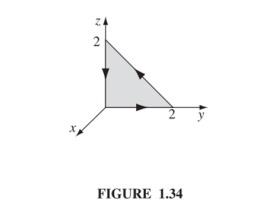
\includegraphics[width=0.5\textwidth]{imagenes/punto_34.jpg} 
    \label{fig:mi_figura}
\end{figure}


Teorema de Stokes
\[
\oint_{\partial S} \mathbf{V} \cdot d\mathbf{l} = \iint_{S} (\nabla \times \mathbf{V}) \cdot d\mathbf{a}
\]

Cálculo del rotacional

\[
\nabla \times \mathbf{V} =
\begin{vmatrix}
\hat{\mathbf{x}} & \hat{\mathbf{y}} & \hat{\mathbf{z}} \\
\frac{\partial}{\partial x} & \frac{\partial}{\partial y} & \frac{\partial}{\partial z} \\
xy & 2yz & 3zx
\end{vmatrix}
\]

\[
= (0 - 2y) \hat{\mathbf{x}} - (3x - 0) \hat{\mathbf{y}} + (0 - x) \hat{\mathbf{z}}
\]

\[
= -2y \hat{\mathbf{x}} - 3x \hat{\mathbf{y}} - x \hat{\mathbf{z}}
\]

Área diferencial:

\[
d\mathbf{a} = dy dz \, \hat{\mathbf{x}}
\]

\[
(\nabla \times \mathbf{V}) \cdot d\mathbf{a} = (-2y) dy dz
\]

Por tanto:

\[
\iint_S -2y \, dy dz
\]

\[
\int_2^0 \int_2^{2+z} -2y \, dy dz
\]

Para los límites de \( y \):

\[
m = \frac{z_2 - z_1}{y_2 - y_1} = \frac{2 - 0}{0 - 2} = -1
\]
\[
 z- z_1=m({y - y_1} )
\]
\[
z - 0 = m(y - 2)
\]

\[
z - 0 = -1(y - 2)
\]

\[
z = -1y + 2
\]

\[
y = 2 - z
\]

Resolviendo la integral:
\begin{align*}
    \int_0^2 dz \int_0^{2-z} (-2y) dy &= \int_0^2 dz \left[ -y^2 \right]_0^{2-z} \\
    &= \int_0^2 dz \left( - (2-z)^2 \right) \\
    &= \int_0^2 dz (-4 + 4z - z^2) \\
    &= \left[ -4z + 2z^2 - \frac{z^3}{3} \right]_0^2 \\
    &= \left( -8 + 8 - \frac{8}{3} \right) \\
    &=\boxed{ -\frac{8}{3}}
\end{align*}
Por otro lado:
\[
\oint_{\partial S} \mathbf{V} \cdot d\mathbf{l} 
\] 
La parametrización de la curva se realiza dividiéndola en tres segmentos:
\[
\lambda = \lambda_1 + \lambda_2 + \lambda_3
\]


Para el segmento en la dirección de $\hat{y}$, se tiene:

\[
y: 0 \to 1
\]

Dado que $dx = dz = 0$, entonces la integral en este tramo es:

\[
\int = 0
\]

Para el siguiente segmento, con $x = 0$:

\[
dx = 0
\]
\[
y = 2 - z
\]
\[
dy = -dz
\]

Evaluado la integral:

\[
\int 2 yz \, dy
\]

Reescribiendo la integral en términos de $z$:

\[
-\int_0^2 2(2 - z)z \, dz
\]

Desarrollando:

\[
-\int_0^2 (4z - 2z^2) \, dz
\]

\[
-\left[ \frac{4z^2}{2} - \frac{2z^3}{3} \right]_0^2
\]

\[
=-\left[ \frac{8}{2} - \frac{16}{3} \right]
\]

\[
=-\left( \frac{24 - 16}{3} \right)
\]

\[
\boxed{ =-\frac{8}{3}}
\]
\section*{\question{Problema  1.36}} Demuestre que:

(a) 
\[
\int_S f (\nabla \times A) \cdot da = \int_S [ A \times (\nabla f)] \cdot da + \oint_p f A \cdot dl
\]

(b) 
\[
\int_V b \cdot (\nabla \times A) d\tau = \int_V A \cdot (\nabla \times B) d\tau + \int_S (A \times B) \cdot da
\]

\textbf{Solución (a)}

Usando la identidad

\[
\nabla \times (f A) = f (\nabla \times A) + (\nabla f) \times A
\]

Usando Stokes:

\[
\int_S \nabla \times (f A) \cdot da = \oint_p f A \cdot dl
\]

\[
\int_S [ f (\nabla \times A) + (\nabla f) \times A ] \cdot da = \oint_p f A \cdot dl
\]

Separando la integral:

\[
\int_S f (\nabla \times A) \cdot da + \int_S [ (\nabla f) \times A ] \cdot da = \oint_p f A \cdot dl
\]

Organizando:

\[
\int_S f (\nabla \times A) \cdot da = \int_S [ A \times (\nabla f)] \cdot da + \oint_p f A \cdot dl
\]

\textbf{Solución (b)}
Usando la identidad:

\[
\nabla \cdot ( A \times B ) = B \cdot (\nabla \times A) - A \cdot (\nabla \times B)
\]

Teorema de la divergencia:
\[
\int_V \nabla \cdot (A \times B) d\tau = \int_S (A \times B) \cdot da
\]

\[
\int_V \left[ B \cdot (\nabla \times A) - A \cdot (\nabla \times B) \right] d\tau = \int_S (A \times B) \cdot da
\]

\[
\int_V B \cdot (\nabla \times A) d\tau - \int_V A \cdot (\nabla \times B) d\tau = \int_S (A \times B) \cdot da
\]

Reorganizo:

\[
\int_V B \cdot (\nabla \times A) d\tau = \int_V A \cdot (\nabla \times B) d\tau + \int_S (A \times B) \cdot da
\]
\section*{\question{Problema  1.38} }Exprese los vectores unitarios \( \hat{r}, \hat{\theta}, \hat{\varphi} \) en términos de \( \hat{x}, \hat{y}, \hat{z} \) y después deduzca la ec. 1.64.  Verifíque la respuesta de varias maneras \(\hat{r}\cdot\hat{r}= 1, \hat{r}\cdot\hat{\theta}= 0, r\hat{r}\cdot\hat{\phi}= 0, etc.\). También encontrar las fórmulas inversas, dando \( \hat{x}, \hat{y}, \hat{z} \) en términos de \( \hat{r}, \hat{\theta}, \hat{\varphi} \).

\[
r = x \hat{x} + y \hat{y} + z \hat{z}
\]

\[
x = r \sin\theta \cos\varphi
\]

\[
y = r \sin\theta \sin\varphi
\]

\[
z = r \cos\theta
\]

\[
\hat{r} = r\sin\theta \cos\varphi \hat{x} + r\sin\theta \sin\varphi \hat{y} + r\cos\theta \hat{z}
\]

\[
\hat{r}= \frac{ \frac{\partial r}{\partial r}}
{| \frac{\partial r}{\partial r}  |}
\]

\[
\frac{\partial r}{\partial r} = \sin\theta \cos\varphi \hat{x} + \sin\theta \sin\varphi \hat{y} + \cos\theta \hat{z}
\]

\[
\left| \frac{\partial r}{\partial r} \right| = \sqrt{\sin^2\theta \cos^2\varphi + \sin^2\theta \sin^2\varphi + \cos^2\theta} 
\]
\[
= \sqrt{1} = 1
\]

\[
\boxed{\hat{r} = \sin\theta \cos\varphi \hat{x} + \sin\theta \sin\varphi \hat{y} + \cos\theta \hat{z}}
\]

Para \( \hat{\theta} \):

\[
\hat{\theta} = \frac{\frac{dr}{d\theta}}{\left| \frac{dr}{d\theta} \right|}
\]

\[
\frac{dr}{d\theta} = r \cos\theta \cos\varphi \hat{x} + r \cos\theta \sin\varphi \hat{y} - r \sin\theta \hat{z}
\]

\[
\left| \frac{dr}{d\theta} \right| = r \sqrt{\cos^2\theta (\cos^2\varphi + \sin^2\varphi) + \sin^2\theta}
\]

\[
= r \sqrt{\cos^2\theta + \sin^2\theta} = r
\]

\[
\boxed{\hat{\theta} = \cos\theta \cos\varphi \hat{x} + \cos\theta \sin\varphi \hat{y} - \sin\theta \hat{z}}
\]


Para \( \hat{\varphi} \):

\[
\hat{\varphi} = \frac{\frac{dr}{d\varphi}}{\left| \frac{dr}{d\varphi} \right|}
\]

\[
\frac{dr}{d\varphi} = -r \sin\theta \sin\varphi \hat{x} + r \sin\theta \cos\varphi \hat{y}
\]

\[
\left| \frac{dr}{d\varphi} \right| = r \sqrt{\sin^2\theta \sin^2\varphi + \sin^2\theta \cos^2\varphi}
\]

\[
\left| \frac{dr}{d\varphi} \right|= r \sin\theta
\]
\[
\boxed{\hat{\varphi} = -\sin\varphi \hat{x} + \cos\varphi \hat{y}}
\]



Comprobando la respuesta:
\[
\hat{r} \cdot \hat{r} = \sin^2\theta (\cos^2\phi + \sin^2\phi) + \cos^2\theta = \sin^2\theta + \cos^2\theta = 1 \quad \checkmark
\]
\[
\hat{\theta} \cdot \hat{\phi} = -\cos\theta \sin\phi \cos\phi + \cos\theta \sin\phi \cos\phi = 0 \quad \checkmark 
\]
Ahora, para  las fórmulas inversas, dejando \( \hat{x}, \hat{y}, \hat{z} \) en términos de \( \hat{r}, \hat{\theta}, \hat{\varphi} \).


\[
\sin\theta \hat{r} = \sin^2\theta \cos\phi \hat{x} + \sin^2\theta \sin\phi \hat{y} + \sin\theta \cos\theta \hat{z}.
\]

\[
\cos\theta \hat{\theta} = \cos^2\theta \cos\phi \hat{x} + \cos^2\theta \sin\phi \hat{y} - \sin\theta \cos\theta \hat{z}.
\]

Añadiendo estas ecuaciones:

\begin{enumerate}
    \item $\sin\theta \hat{r} + \cos\theta \hat{\theta} = +\cos\phi \hat{x} + \sin\phi \hat{y}$
    \item $\hat{\phi} = -\sin\phi \hat{x} + \cos\phi \hat{y}$
\end{enumerate}

Multiplicando (1) por $\cos\phi$, (2) por $\sin\phi$ y restando:

\[
\boxed{\hat{x} = \sin\theta \cos\phi \hat{r} + \cos\theta \cos\phi \hat{\theta} - \sin\phi \hat{\phi}.}
\]

Multiplicando (1) por $\sin\phi$, (2) por $\cos\phi$ y sumando:

\[
\boxed{\hat{y} = \sin\theta \sin\phi \hat{r} + \cos\theta \sin\phi \hat{\theta} + \cos\phi \hat{\phi}.}
\]

\[
\cos\theta \hat{r} = \cos\theta \sin\theta \cos\phi \hat{x} + \cos\theta \sin\theta \sin\phi \hat{y} + \cos^2\theta \hat{z}.
\]

\[
\sin\theta \hat{\theta} = \sin\theta \cos\theta \cos\phi \hat{x} + \sin\theta \cos\theta \sin\phi \hat{y} - \sin^2\theta \hat{z}.
\]

Restando estas ecuaciones:

\[
\boxed{\hat{z} = \cos\theta \hat{r} - \sin\theta \hat{\theta}.}
\]


%-----------------------------------------EJ_1_IDMCH-----------------------------------------    
\section*{\color{blue} Problema 1.40}
Calcule la divergencia de la función  
\[
\mathbf{v} = (r\cos\theta)\,\hat{\mathbf{r}} + (r\sin\theta)\,\hat{\boldsymbol{\theta}} + (r\sin\theta\cos\phi)\,\hat{\boldsymbol{\phi}}.
\]  
Verifique el teorema de la divergencia para esta función, utilizando como volumen el casquete semiesférico invertido de radio \(R\), apoyado en el plano \(xy\) y centrado en el origen (Figura 1.40).
\begin{figure}[ht]
    \centering
    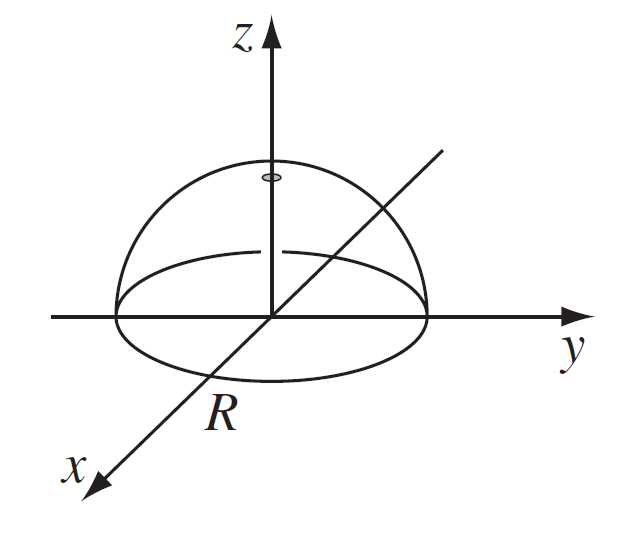
\includegraphics[width=0.5\textwidth]{imagenes/punto_40.png}
    \captionsetup{labelformat=empty}
    \caption{Figura 1.40: casquete semiesférico}
\end{figure}

\subsection*{Solución}
\paragraph*{Cálculo de la divergencia}  
En coordenadas esféricas, la divergencia de \(\mathbf{v}\) es:  
\[
\nabla \cdot \mathbf{v} = \frac{1}{r^2} \frac{\partial}{\partial r} \left( r^2 v_r \right) + \frac{1}{r\sin\theta} \frac{\partial}{\partial \theta} \left( \sin\theta \, v_\theta \right) + \frac{1}{r\sin\theta} \frac{\partial v_\phi}{\partial \phi}.
\]  
Sustituyendo \(v_r = r\cos\theta\), \(v_\theta = r\sin\theta\), \(v_\phi = r\sin\theta\cos\phi\):  
\[
\nabla \cdot \mathbf{v} = \frac{1}{r^2} \frac{\partial}{\partial r} \left( r^3 \cos\theta \right) + \frac{1}{r\sin\theta} \frac{\partial}{\partial \theta} \left( r\sin^2\theta \right) + \frac{1}{r\sin\theta} \frac{\partial}{\partial \phi} \left( r\sin\theta\cos\phi \right).
\]  
Simplificando:  
\[
\nabla \cdot \mathbf{v} = 3\cos\theta + 2\cos\theta - \sin\phi = 5\cos\theta - \sin\phi.
\]
\[
\nabla \cdot \mathbf{v} = 5\cos\theta - \sin\phi.
\]

\paragraph*{Verificación del teorema de la divergencia} 

El casquete semiesférico está dado por:
\[0 \leq r \leq R\] \[0 \leq \theta \leq \pi/2\] \[0 \leq \phi \leq 2\pi\ \]   

1. \textbf{Integral de volumen de \(\nabla \cdot \mathbf{v}\):}  
\[
\int_V (\nabla \cdot \mathbf{v}) \, dV = \int_0^R \int_{0}^{\pi/2} \int_0^{2\pi} \left( 5\cos\theta - \sin\phi \right) r^2 \sin\theta \, d\phi \, d\theta \, dr.
\]  
El término \(\sin\phi\) se anula al integrar en \(\phi\) debido a la paridad:  
\[ \int_{0}^{2\pi} r^2\sin\theta\sin\phi \, d\phi = 0\]

Por lo tanto, la integral que queda es:

\begin{align*}
    \int_V (\nabla \cdot \mathbf{v}) \, dV & = \int_{0}^{2\pi} d\phi \int_0^R r^2 \, dr \int_{0}^{\pi/2} 5\cos\theta \sin\theta \, d\theta\\
& = \frac{R^3}{3} 10\pi \int_{0}^{\pi/2} \sin\theta\cos\theta \,d\theta    \\    
& = \frac{10\pi R^3}{3}\frac{1}{2} \\    
& = \frac{5\pi R^3}{3}.
\end{align*}

2. \textbf{Integral de línea a través de la tapa y de la semiesfera:} 
 
\[
\oint_{c_1} \mathbf{v} \cdot d\mathbf{a} + \oint_{c_2}\mathbf{v} \cdot d\mathbf{a} 
\]  

- \textbf{Flujo sobre el circulo de radio \(R\)}:
\[\oint_{c_1} \mathbf{v} \cdot d\mathbf{a}\]
donde 
\[\theta = \pi/2 \,, \phi:0 \rightarrow 2\pi \,, r:0 \rightarrow R\]
El diferencial de área del circulo es: 

\[d\mathbf{a} = r\sin\theta \, d\phi \, dr\, \hat{\theta }\] con \(\theta = \pi/2\) 
\[d\mathbf{a} = r \, d\phi \, dr\, \hat{\theta }\]

\begin{align*}
\oint_{c_1 } \mathbf{v} \cdot d \mathbf{a}  = & \oint_{c_1} ((r\cos\theta)\,\hat{\mathbf{r}} + (r\sin\theta)\,\hat{\boldsymbol{\theta}} + (r\sin\theta\cos\phi)\,\hat{\boldsymbol{\phi}})\cdot(r \, d\phi \, dr\, \hat{\theta }) \\
 = & \oint_{c_1} r^2\sin\theta \, d\phi \, dr \\
 = & \oint_{c_1} r^2 \, d\phi \, dr \\
 = & \int_{0}^{2\pi} \, d\phi \int_{0}^{R} r^2 \, dr \\
 = & \boxed{2\pi \frac{R^3}{3}} .
\end{align*}

- \textbf{Flujo sobre la superficie de la semiesfera}:
\[\oint_{c_2} \mathbf{v} \cdot d\mathbf{a}\]
donde 
\[\theta :0 \rightarrow\pi/2 \,, \phi:0 \rightarrow 2\pi \,, r = R\]
el diferencial de área de la superficie semiesférica es: 

\[d\mathbf{a} = r^2\sin\theta \, d\phi \, d\theta\, \hat{\phi }\] con \(r = R\) 
\[d\mathbf{a} = R^2 \sin\theta \, d\phi \, d\theta\, \hat{\theta }\]

\begin{align*}
\oint_{c_2 } \mathbf{v} \cdot d \mathbf{a}  &= \oint_{c_2} ((r\cos\theta)\,\hat{\mathbf{r}} + (r\sin\theta)\,\hat{\boldsymbol{\theta}} + (r\sin\theta\cos\phi)\,\hat{\boldsymbol{\phi}})\cdot(R^2 \sin\theta \, d\phi \, d\theta\, \hat{\theta }) \\
& = \oint_{c_2} R^3\cos\theta \sin\theta \, d\phi \, d\theta \\
& = R^3 \int_{0}^{2\pi} \, d\phi \int_{0}^{\pi/2} \cos\theta \sin\theta \, d\theta \\
& = R^3 2\pi \frac{1}{2} \\
& = \pi R^3
\end{align*}

Flujo total:  

\[
\frac{2\pi R^3}{3} + \pi R^3 = \boxed{\frac{5\pi R^3}{3}}.
\]  
%-----------------------------------------EJ_2_IDMCH-----------------------------------------    
\section*{\color{blue} Problema 1.42}
\textbf{Problema 1.42} Exprese los vectores unitarios en coordenadas cilíndricas \(\hat{\rho}\), \(\hat{\phi}\), \(\hat{z}\) en términos de \(\hat{x}\), \(\hat{y}\), \(\hat{z}\) (es decir, derive la ecuación 1.75). ``Invierta'' sus fórmulas para obtener \(\hat{x}\), \(\hat{y}\), \(\hat{z}\) en términos de \(\hat{s}\), \(\hat{\phi}\), \(\hat{z}\) (y \(\phi\)).

\begin{figure}[H]
    \centering
    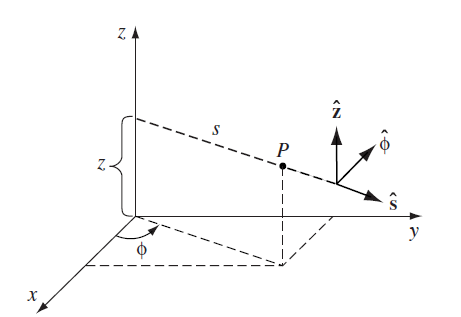
\includegraphics[width=0.5\textwidth]{imagenes/punto_42.png} 
    \captionsetup{labelformat=empty}
    \caption{Figura 42}
\end{figure}

\subsection*{ Solución }
De la imagen 42 se tiene que \(\) se puede expresar como:
\[ \hat{\rho} = \cos\phi\hat{x}  + \sin\phi\hat{y} \]
De la misma forma se tiene que \(\hat{\phi} \)
\[ \hat{\phi} = -\sin\phi\hat{x}  + \cos\phi\hat{y} \]
y \(\hat{z}\) es igual a \(\hat{z}\).\\

por lo tanto  los vectores unitarios en coordenadas cilíndricas \(\hat{\rho}\), \(\hat{\phi}\), \(\hat{z}\) en términos de \(\hat{x}\), \(\hat{y}\), \(\hat{z}\) son:

\begin{align*}
\hat{\rho} &= \cos\phi\hat{x}  + \sin\phi\hat{y} \\
\hat{\phi} &= -\sin\phi\hat{x}  + \cos\phi\hat{y} \\
\hat{z}  & = \hat{z}
\end{align*}

Multiplicando  a \(\hat{\rho} \) por \(\cos \phi\)  y a \(\hat{\phi} \)  por \(\sin \phi\) y luego restando se tiene:


\begin{align*}
\hat{\rho} \cos \phi - \hat{\phi} \sin \phi &= \cos^2 \phi \hat{x} + \cos \phi \sin \phi \hat{y} + \sin^2 \phi \hat{x} - \sin \phi \cos \phi \hat{y} \\
&= \hat{x}(\sin^2 \phi + \cos^2 \phi) \\
&= \hat{x}.
\end{align*}

Por lo tanto,  
\[
\hat{x} = \cos \phi \,\hat{\rho} - \sin \phi \,\hat{\phi}.
\]

Multiplicando  a \(\hat{\phi} \) por \(\cos \phi\)  y a \(\hat{\rho} \)  por \(\sin \phi\) y luego sumando se tiene:
\begin{align*}
\hat{\rho} \sin \phi + \hat{\phi} \cos \phi &= \sin \phi \cos \phi \hat{x} + \sin^2 \phi \hat{y} - \sin \phi \cos \phi \hat{x} + \cos^2 \phi \hat{y} \\
&= \hat{y}(\sin^2 \phi + \cos^2 \phi) \\
&= \hat{y}.
\end{align*}

Por lo tanto,  
\[
\hat{y} = \sin \phi \,\hat{\rho} + \cos \phi \,\hat{\phi}
\]

Por lo tanto  los vectores unitarios en coordenadas cartesianas  \(\hat{x}\), \(\hat{y}\), \(\hat{z}\) en términos de \(\hat{\rho}\), \(\hat{\phi}\), \(\hat{z}\) son:

\begin{align*}
\hat{x} &= \cos\phi\hat{\rho} -\sin\phi\hat{\phi}   \\
\hat{y} &= \sin\phi\hat{\rho}  + \cos\phi\hat{\phi} \\
\hat{z} &= \hat{z}
\end{align*}
%-----------------------------------------EJ_3_IDMCH-----------------------------------------    
\section*{\color{blue} Problema 1.44}
Evalué las siguientes integrales: 
\begin{enumerate}[(a)]
    \item \[
\int_{2}^{6} \bigl(3x^2 - 2x - 1\bigr)\,\delta(x - 3)\,dx
\]
La función delta  evalúa la función en \(x = 3\), por lo tanto:
\[
\int_{2}^{6} \bigl(3x^2 - 2x - 1\bigr)\,\delta(x - 3)\,dx = 3(3)^2 - 2(3) - 1 = 27 - 6 - 1 = \boxed{20}.
\]
    \item \[
 \int_{0}^{5} \cos x \,\delta(x - \pi)\,dx
\]
La función delta  evalúa la función en \(x = \pi\), por lo tanto:
\[
\int_{0}^{5} \cos x \,\delta(x - \pi)\,dx = \cos(\pi) = \boxed{-1} .
\]
    \item \[
 \int_{0}^{3} x^3\,\delta(x + 1)\,dx
  \]
La función delta evalúa la función en \(x = -1\), pero el intervalo de integración no incluye \(x = -1\), por lo tanto:
\[
\int_{0}^{3} x^3\,\delta(x + 1)\,dx = \boxed{0}.
\]
    \item \[
\int_{-\infty}^{\infty} ln(x+3)\,\delta(x+2)\,dx
\]
La función delta evalúa la función en \(x =-2\), por lo tanto:
\[
\int_{-\infty}^{\infty} ln(x+3)\,\delta(x+2)\,dx = ln(-2+3) = ln(1)=\boxed{0}.
\]
\end{enumerate}

%-----------------------------------------EJ_4_IDMCH-----------------------------------------
\section*{\color{blue} Problema 1.46}
\begin{enumerate}[(a)]
    \item Demostrar que:
\[ x \frac{d}{dx}(\delta{(x)})= -\delta{(x)} \]
\subsection*{Solución}
Multiplicando por una función \(f(x)\) y luego integrando en el intervalo \([-\infty,\infty]\):
\[
\int_{-\infty}^{\infty} f(x)\,x \frac{d}{dx}(\delta{(x)}) = -\int_{-\infty}^{\infty} f(x)\,\delta(x).
\]
Integrando por partes:
\[ u = x f(x) \, , du=f(x)+x \frac{df(x)}{dx} \]
\[
 dv = \frac{d}{dx}(\delta(x)) \,, v=\delta(x) \]
\[
\int_{-\infty}^{\infty} f(x)\,x \frac{d}{dx}(\delta{(x)}) =  f(x)\,x \delta(x)|_ {-\infty}^{\infty} - \int_{-\infty}^{\infty} (f(x)+f'(x)\,x) \delta(x) \,dx.
\]
El primer término se anula, por lo tanto:
\[
\int_{-\infty}^{\infty} f(x)\,x \frac{d}{dx}(\delta{(x)}) = -\int_{-\infty}^{\infty} (f(x)+f'(x)\,x )\delta(x) \,dx
\]
La función delta evalúa la función en \(x = 0\), por lo tanto:

\[
-\int_{-\infty}^{\infty} (f(x)+f'(x)\,x) \delta(x) \,dx = -f(0).
\]

\[
\int_{-\infty}^{\infty} f(x)\,x \frac{d}{dx}(\delta{(x)}) = -f(0).
\]
Por lo tanto:
\[
\int_{-\infty}^{\infty} f(x)\,x \frac{d}{dx}(\delta{(x)}) = -\int_{-\infty}^{\infty} f(x)\,\delta(x).
\]
\[\boxed{ x \frac{d}{dx}(\delta{(x)})= -\delta{(x)} }\]

    \item sea \(\theta(x)\) la función escalón :    
 
\[
\theta(x) \equiv
\begin{cases}
1, & \text{if } x > 0,\\
0, & \text{if } x \le 0.
\end{cases}
\]
 muestre que \[\frac{d\theta}{dx} =\delta(x)\]

\subsection*{Solución}
Multiplicando por una función \(f(x)\) y luego integrando en el intervalo \([-\infty,\infty]\):
\[
 \int_{-\infty}^{\infty} f(x) \, \frac{d}{dx}(\theta(x))dx = \int_{-\infty}^{\infty} f(x
) \, \delta(x) \, dx    
\]
integrando por partes 
\[ u = f(x) \, , du=f'(x) \]
\[ dv = \frac{d}{dx}(\theta(x)) \,, v=\theta(x) \]
\[
 \int_{-\infty}^{\infty} f(x) \, \frac{d}{dx}(\theta(x)) dx=  f(x) \, \theta(x)|_
{-\infty}^{\infty} - \int_{-\infty}^{\infty} f'(x) \, \theta(x) \, dx
\]


Evaluando los  términos de frontera:
   \[
   \left[ f(x) \Theta(x) \right]_{-\infty}^{\infty} = f(\infty) \cdot 1 - f(-\infty) \cdot 0
   \]
    Dado que la función \( f(x) \)  (se anula en \( x \to \pm\infty \)):
   \[
   f(\infty) = 0 \quad \text{y} \quad f(-\infty) = 0
   \]
   Por lo tanto:
   \[
   \left[ f(x) \Theta(x) \right]_{-\infty}^{\infty} = 0 - 0 = 0
   \]

Simplificando  la integral restante:
   \[
    -\int_{-\infty}^{\infty} \Theta(x) f'(x) \, dx 
   \]
    Como \( \Theta(x) = 0 \) para \( x \leq 0 \), la integral se reduce a:
   \[
   - \int_{0}^{\infty} f'(x) \, dx 
   \]
    Integrando \( f'(x) \):
   \[
   \left[ f(x) \right]_{0}^{\infty} = - \left( 0{f(\infty)} - f(0) \right) = f(0)
   \]

   \[
   \int_{-\infty}^{\infty} f(x) \frac{d\Theta}{dx} \, dx = f(0)
   \]
   - Esto coincide con la propiedad de la delta de Dirac:
   \[
   \int_{-\infty}^{\infty} f(x) \delta(x) \, dx = f(0)
   \]

por lo tanto:
\[\boxed{\frac{d\theta}{dx} =\delta(x)}\]

\end{enumerate}
%-----------------------------------------EJ_5_IDMCH-----------------------------------------
\section*{\color{blue} Problema 1.48}

Evaluar las siguientes integrales:
\begin{enumerate}[(a)]

    \item 
    \[
    \int \bigl(r^2 + \mathbf{r}\cdot\mathbf{a} + a^2\bigr)\,\delta^3(\mathbf{r} - \mathbf{a}) \, d\tau,
    \]
    donde \(\mathbf{a}\) es un vector fijo, \(a = \|\mathbf{a}\|\) es su magnitud, y la integral se realiza sobre todo el espacio.
    
    La delta en 3 dimensiones evalúa la función en \(\mathbf{r} = \mathbf{a}\), por lo tanto:
    \[
    \int \bigl(r^2 + \mathbf{a}\cdot\mathbf{a} + a^2\bigr)\,\delta^3(\mathbf{r} - \mathbf{a}) \, d\tau = a^2 + \mathbf{a}\cdot \mathbf{a}   + a^2 = \boxed{3a^2}.
    \]
    \item 
    \[
    \int_V \bigl(\mathbf{r} - \mathbf{b}\bigr)^2 \,\delta^3(5\mathbf{r}) \, d\tau,
    \]
    donde \(V\) es un cubo de lado 2, centrado en el origen, y \(\mathbf{b} = 4\,\hat{\mathbf{y}} + 3\,\hat{\mathbf{z}}\).

    Primero expresamos la delta como:

    \[ \delta(5 \mathbf{r} )= \frac{1}{5^3}\delta(\mathbf{r} ) \]
    la integral queda:
    \[
    \int_V \bigl(\mathbf{r} - \mathbf{b}\bigr)^2 \,\frac{1}{5^3} \delta^3(\mathbf{r}) \, d\tau,
    \]
    La delta en 3 dimensiones evalúa la función en \(\mathbf{r} = 0\), por lo tanto:
    \[ \int_V \bigl(\mathbf{r} - \mathbf{b}\bigr)^2 \,\frac{1}{5^3} \delta^3(\mathbf{r}) \, d\tau = \frac{\mathbf{(b)^2} }{5^3}  \]
    remplazando \(\mathbf{b}= 4\,\hat{\mathbf{y}} + 3\,\hat{\mathbf{z}}\) se tiene:
    \begin{align*}
        \frac{\mathbf{(b)^2} }{5^3} &= \frac{(4\,\hat{\mathbf{y}} + 3\,\hat{\mathbf{z}})^2}{5^3}\\
    & =\frac{4^2+3^2}{5^3} \\
    & =\frac{16+9}{125} \\
    & =\frac{25}{125} \\
    & =\boxed{\frac{1}{5}}
    \end{align*}
   
    \item 
    \[
    \int_V \bigl[r^4 + r^2\,(\mathbf{r}\cdot\mathbf{c}) + c^4\bigr]\,
    \delta^3(\mathbf{r} - \mathbf{c}) \, d\tau,
    \]
    donde \(V\) es una esfera de radio 6 centrada en el origen, \(\mathbf{c} = 5\,\hat{\mathbf{x}} + 3\,\hat{\mathbf{y}} + 2\,\hat{\mathbf{z}}\) y \(c = \|\mathbf{c}\|\) es su magnitud.
    
    La delta en 3 dimensiones evalúa la función en \(\mathbf{r} = \mathbf{c}\), pero la magnitud de $\mathbf{c}$  debe de estar dentro de la esferea de radio 6:
    \[|\mathbf{c} |= (5^2+3^2+2^2) = 38 \,, 38 > 6^2\]
    Por lo tanto la integral es cero.
    \[\int_V \bigl[r^4 + r^2\,(\mathbf{r}\cdot\mathbf{c}) + c^4\bigr]\,
    \delta^3(\mathbf{r} - \mathbf{c}) \, d\tau = \boxed{0} \]


    \item 
    \[
    \int_V \bigl[\mathbf{r} \cdot (\mathbf{d} - \mathbf{r})\bigr]\,
    \delta^3(\mathbf{e} - \mathbf{r}) \, d\tau,
    \]
    donde \(\mathbf{d} = (1,2,3)\), \(\mathbf{e} = (3,2,1)\) y \(V\) es una esfera de radio 1.5 centrada en \((2,2,2)\).
    encontrando si \(\mathbf{e} \) se encuentra dendtro de la esferea de radio 1.5 centrada en \((2,2,2)\):
    \[(\mathbf{e} - (2,2,2))^2 = (3-2,2-2,1-2)^2 = (1,0,-1)^2 = 2 <(1.5)^2\]
    por lo tanto se encuentra dentro de la esfera.\\
    Expresamos la delta como:
    \[ \delta(\mathbf{e} - \mathbf{r} )= \delta(\mathbf{r} - \mathbf{e} ) \]
    la integral queda:
    \[
    \int_V \bigl[\mathbf{r} \cdot (\mathbf{d} - \mathbf{r})\bigr]\,
    \delta^3(\mathbf{r} - \mathbf{e}) \, d\tau
    \]
    La delta evalúa la función en \(\mathbf{r} = \mathbf{e}\), por lo tanto:
    \begin{align*}
        \int_V \bigl[\mathbf{r} \cdot (\mathbf{d} - \mathbf{r})\bigr]\,
        \delta^3(\mathbf{r} - \mathbf{e}) \, d\tau& = = \mathbf{e} \cdot (\mathbf{d} - \mathbf{e}).\\
& = (3,2,1)\cdot((1,2,3)-(3,2,1))\\ 
& = (3,2,1)\cdot(-2,0,2)\\
& = -6+0+2\\
& = \boxed{-4}
    \end{align*}
    
    \end{enumerate}
%-----------------------------------------EJ_6_IDMCH-----------------------------------------
\section*{\color{blue} Problema 1.50}
\begin{enumerate}[(a)]
    \item  
    Sea \(
    \mathbf{F}_1 = x^2 \,\hat{\mathbf{z}}, 
    \quad
    \mathbf{F}_2 = x\,\hat{\mathbf{x}} + y\,\hat{\mathbf{y}} + z\,\hat{\mathbf{z}}.
    \)
    Calcule la \emph{divergencia} y el \emph{rotacional} de \(\mathbf{F}_1\) y \(\mathbf{F}_2\). 
    
    \noindent
    ¿Cuál de ellas puede escribirse como el gradiente de un escalar? Encuentre un potencial escalar que lo demuestre. 
    
    \noindent
    ¿Cuál puede escribirse como el rotacional de un vector? Encuentre un potencial vectorial adecuado.
    \subsection*{Solución}


    \textbf{Divergencia de \(\mathbf{F} _1\):}
    \[
    \nabla \cdot \mathbf{F} _1 = \frac{\partial (0)}{\partial x} + \frac{\partial (0)}{\partial y} + \frac{\partial (x^2)}{\partial z} = .
    \]
    \[
    \boxed{\nabla \cdot \mathbf{F} _1 = 0.}
    \]

    \textbf{Divergencia de \(\mathbf{F} _2\):}
    \[
    \nabla \cdot \mathbf{F} _2 = \frac{\partial (x)}{\partial x} + \frac{\partial (y)}{\partial y} + \frac{\partial (z)}{\partial z} = 1 + 1 + 1 = 3.
    \]
    \[
    \boxed{\nabla \cdot \mathbf{F} _2 = 3.}
    \]
    \textbf{Rotacional de \(\mathbf{F} _1\):}
    \[
    \nabla \times \mathbf{F} _1 = \begin{vmatrix}
    \hat{x} & \hat{y} & \hat{z} \\
    \frac{\partial}{\partial x} & \frac{\partial}{\partial y} & \frac{\partial}{\partial z} \\
    0 & 0 & x^2
    \end{vmatrix} = \hat{x} \left(\frac{\partial (x^2)}{\partial y} - \frac{\partial (0)}{\partial z}\right) - \hat{y} \left(\frac{\partial (x^2)}{\partial x} - \frac{\partial (0)}{\partial z}\right) + \hat{z} \left(\frac{\partial (0)}{\partial x} - \frac{\partial (0)}{\partial y}\right) = \boxed{-2x \hat{y}.}
    \]


    \textbf{Rotacional de \(\mathbf{F} _2\):}
    \[
    \nabla \times \mathbf{F} _2 = \begin{vmatrix}
    \hat{x} & \hat{y} & \hat{z} \\
    \frac{\partial}{\partial x} & \frac{\partial}{\partial y} & \frac{\partial}{\partial z} \\
    x & y & z
    \end{vmatrix} = \hat{x} \left(\frac{\partial z}{\partial y} - \frac{\partial y}{\partial z}\right) - \hat{y} \left(\frac{\partial z}{\partial x} - \frac{\partial x}{\partial z}\right) + \hat{z} \left(\frac{\partial y}{\partial x} - \frac{\partial x}{\partial y}\right) = \boxed{0}.
    \]

    \(\mathbf{F_1}\) tiene divergencia nula, por lo tanto puede expresarse como el rotacional de una función vectorial.
    \[\mathbf{F_1} = \nabla X \mathbf{A_1}  \]
    Dado que \(\mathbf{F_1}\) solo tiene componente en \(\hat{z} \,, \hat{x}=\hat{y}=0\), la función se puede expresar como:
    \[x^2 \hat{z} = \left( \frac{\partial A_y}{\partial x} -\frac{\partial A_x}{\partial y}  \right)\hat{z} \]
    el termino de \(A_  y\) es cero, por lo tanto:
    \[x^2  = \frac{\partial A_y}{\partial x} \]
    integrando:
    \[A_y = \frac{1}{3}x^3 \]
    por lo tanto el potencial vectorial es:
    \[
    \boxed{\phi_2 = \frac{1}{3}x^3 \hat{y}.}
    \]

    
    \(\mathbf{F_2}\) tiene Rotacional nulo, por lo tanto puede expresarse como el gradiente de un escalar.\\
    \[\mathbf{F_2} = -\nabla\phi_2 \]
    Una función escalar que cumple con esto es:
    \[
    \boxed{\phi_2 = \frac{1}{2}x^3 + \frac{1}{2}y^2 + \frac{1}{2}z^2.}
    \]




    \item Muestre que 
    \( \mathbf{F}_3 = zy\,\hat{\mathbf{x}} + zx\,\hat{\mathbf{y}} + xy\,\hat{\mathbf{z}}\)
    puede escribirse tanto como el \emph{gradiente} de un escalar como el \emph{rotacional} de un vector. 
    Encuentre los potenciales escalar y vectorial para esta función.
    \subsection*{Solución}

   
    \[
    \nabla \cdot \mathbf{F_3} = \frac{\partial (yz)}{\partial x} + \frac{\partial (zx)}{\partial y} + \frac{\partial (xy)}{\partial z} = 0 + 0 + 0 = 0.
    \]
    \textbf{Rotacional de \(\mathbf{F_3} \):}
    \[
    \nabla \times \mathbf{F_3}  = \begin{vmatrix}
    \hat{x} & \hat{y} & \hat{z} \\
    \frac{\partial}{\partial x} & \frac{\partial}{\partial y} & \frac{\partial}{\partial z} \\
    yz & zx & xy
    \end{vmatrix} = \hat{x} \left(\frac{\partial (xy)}{\partial y} - \frac{\partial (zx)}{\partial z}\right) - \hat{y} \left(\frac{\partial (xy)}{\partial x} - \frac{\partial (yz)}{\partial z}\right) + \hat{z} \left(\frac{\partial (zx)}{\partial x} - \frac{\partial (yz)}{\partial y}\right) = 0.
    \]


    Además, \(\mathbf{F_3} \) es un campo conservativo, por lo que existe un potencial \(U_3\) tal que \(\mathbf{F_3} = \nabla U_3\). Integrando:
    \[
    \frac{\partial U_3}{\partial x} = yz \implies U_3 = xyz  
    \]
    \[
    \frac{\partial U_3}{\partial y} = zx \implies U_3 = xyz + 
    \]
    \[
    \frac{\partial U_3}{\partial z} = xy \implies U_3 = xyz + 
    \]
    Por tanto, el potencial es 
    \[\boxed{U_3 = xyz}\]
    
De la misma manera  \(\mathbf{F_3} \) se puede escribir como el rotacional de un vector, por lo que existe un campo vectorial \(\mathbf{A_3}\) tal que \(\mathbf{F_3} = \nabla \times \mathbf{A_3}\). Integrando:
    \[
    \frac{\partial A_{3z}}{\partial y} - \frac{\partial A_{3y}}{\partial z} = yz \implies A_{3z} = \frac{1}{2} y^2 z + f_1(x,z)\, 
    \]
    \[
    \frac{\partial A_{3x}}{\partial z} - \frac{\partial A_{3z}}{\partial x} = zx \implies A_{3x} = \frac{1}{2} z^2 y + f_2(x,y)
    \]
    \[
    \frac{\partial A_{3y}}{\partial x} - \frac{\partial A_{3x}}{\partial y} = xy \implies A_{3y} = \frac{1}{2} y x^2 + f_3(y,z)
    \]
    Por tanto, el campo vectorial es 
    \[\boxed{\mathbf{A_3} = \frac{1}{2} z^2 y \hat{\mathbf{x}} + \frac{1}{2} x^2 y \hat{\mathbf{y}} + \frac{1}{2} z y^2 \hat{\mathbf{z}}}\]
\end{enumerate}

%-----------------------------------------EJ_7_IDMCH-----------------------------------------
\section*{\color{blue} Problema 1.52}
Del Teorema 2  

$\mathbf{Campos\, solenoidales}$

\begin{enumerate}
    \item[(a)] \(\nabla \cdot \mathbf{F} = 0\) en todas partes.

    \item[(b)] \(\displaystyle \int \mathbf{F} \cdot d\mathbf{a}\) es independiente de la superficie elegida, para cualquier línea de frontera dada.

    \item[(c)] \(\displaystyle \oint \mathbf{F} \cdot d\mathbf{a} = 0\) para cualquier superficie cerrada.

    \item[(d)] \(\mathbf{F}\) es el rotacional de alguna función vectorial: \(\mathbf{F} = \nabla \times \mathbf{A}\).
\end{enumerate}

 mostrar que \( (d)\Rightarrow (a)\,, (a) \Rightarrow (c)\,, (c)\Rightarrow (b) \,, (b) \Rightarrow (c)\,, (c)\Rightarrow(a)\)
 

\textbf{Demostración }

\begin{enumerate}[(a)]
 \item  (d) \(\Rightarrow\) (a): 
     \[
     \nabla \cdot \mathbf{F} = \nabla \cdot (\nabla \times \mathbf{W}) = 0 \quad \text{( la divergencia de un rotacional siempre es cero).}
     \]
 
\item (a) \(\Rightarrow\) (c):
     \[
     \oint \mathbf{F} \cdot d\mathbf{a} = \int (\nabla \cdot \mathbf{F}) \, d\tau = 0 \quad \text{( teorema de la divergencia).}
     \]
 
\item (c) \(\Rightarrow\) (b):
     \[
     \int_{\text{I}} \mathbf{F} \cdot d\mathbf{a} - \int_{\text{II}} \mathbf{F} \cdot d\mathbf{a} = \oint \mathbf{F} \cdot d\mathbf{a} = 0,
     \]
     por lo tanto:
     \[
     \int_{\text{I}} \mathbf{F} \cdot d\mathbf{a} = \int_{\text{II}} \mathbf{F} \cdot d\mathbf{a}.
     \]
     \textit{ El cambio de signo se debe a que, en \(\oint \mathbf{F} \cdot d\mathbf{a}\), \(d\mathbf{a}\) apunta hacia afuera, mientras que en la superficie II apunta hacia adentro.}
 
\item  (b) \(\Rightarrow\) (c):
     Mismo argumento que (c) \(\Rightarrow\) (b), pero en sentido inverso. \\
\item  (c) \(\Rightarrow\) (a):
     Mismo argumento que (a) \(\Rightarrow\) (c).
\end{enumerate}
\end{document}